\documentclass{article}

\usepackage{fancyhdr}
\usepackage{extramarks}
\usepackage{amsmath}
\usepackage{amsthm}
\usepackage{amsfonts}
\usepackage{tikz}
\usepackage[plain]{algorithm}
\usepackage{algpseudocode}
\usepackage{listings}
\usepackage{xcolor}


\lstset{
	language=Python,
	backgroundcolor=\color{black!5}, % Light background for contrast
	basicstyle=\ttfamily\small, % Font style and size
	keywordstyle=\color{blue}\bfseries, % Blue color for keywords
	commentstyle=\color{green!60!black}\itshape, % Green color for comments, italicized
	stringstyle=\color{red}, % Red color for strings
	numbers=left, % Show line numbers on the left side
	numberstyle=\tiny\color{gray}, % Small, gray numbers
	stepnumber=1, % Number every line
	numbersep=5pt, % Distance between line numbers and code
	frame=single, % Adds a frame around the code
	rulecolor=\color{black}, % Frame color
	captionpos=b, % Caption position at the bottom
	breaklines=true, % Line break for long lines
	breakatwhitespace=true, % Break lines at spaces
	showstringspaces=false, % Don't show space as special character
	morekeywords={lambda, with, as} % Add any extra keywords here
}


\usetikzlibrary{automata,positioning}

%
% Basic Document Settings
%

\topmargin=-0.45in
\evensidemargin=0in
\oddsidemargin=0in
\textwidth=6.5in
\textheight=9.0in
\headsep=0.25in

\linespread{1.1}

\pagestyle{fancy}
\lhead{\hmwkAuthorName}
\chead{\hmwkClass\ (\hmwkClassInstructor): \hmwkTitle}
\rhead{\firstxmark}
\lfoot{\lastxmark}
\cfoot{\thepage}

\renewcommand\headrulewidth{0.4pt}
\renewcommand\footrulewidth{0.4pt}

\setlength\parindent{0pt}

%
% Create Problem Sections
%

\newcommand{\enterProblemHeader}[1]{
	\nobreak\extramarks{}{Problem \arabic{#1} continued on next page\ldots}\nobreak{}
	\nobreak\extramarks{Problem \arabic{#1} (continued)}{Problem \arabic{#1} continued on next page\ldots}\nobreak{}
}

\newcommand{\exitProblemHeader}[1]{
	\nobreak\extramarks{Problem \arabic{#1} (continued)}{Problem \arabic{#1} continued on next page\ldots}\nobreak{}
	\stepcounter{#1}
	\nobreak\extramarks{Problem \arabic{#1}}{}\nobreak{}
}

\setcounter{secnumdepth}{0}
\newcounter{partCounter}
\newcounter{homeworkProblemCounter}
\setcounter{homeworkProblemCounter}{1}
\nobreak\extramarks{Problem \arabic{homeworkProblemCounter}}{}\nobreak{}

%
% Homework Problem Environment
%
% This environment takes an optional argument. When given, it will adjust the
% problem counter. This is useful for when the problems given for your
% assignment aren't sequential. See the last 3 problems of this template for an
% example.
%
\newenvironment{homeworkProblem}[1][-1]{
	\ifnum#1>0
		\setcounter{homeworkProblemCounter}{#1}
	\fi
	\section{Problem \arabic{homeworkProblemCounter}}
	\setcounter{partCounter}{1}
	\enterProblemHeader{homeworkProblemCounter}
}{
	\exitProblemHeader{homeworkProblemCounter}
}

%
% Homework Details
%   - Title
%   - Due date
%   - Class
%   - Section/Time
%   - Instructor
%   - Author
%

\newcommand{\hmwkTitle}{Asignacion\ \#1a}
\newcommand{\hmwkDueDate}{March 25, 2025}
\newcommand{\hmwkClass}{ESMA 5015}
\newcommand{\hmwkClassInstructor}{Damaris Santana}
\newcommand{\hmwkAuthorName}{\textbf{Alejandro Ouslan}}

%
% Title Page
%

\title{
	\vspace{2in}
	\textmd{\textbf{\hmwkClass:\ \hmwkTitle}}\\
	\normalsize\vspace{0.1in}\small{Due\ on\ \hmwkDueDate}\\
	\vspace{0.1in}\large{\textit{\hmwkClassInstructor}}
	\vspace{3in}
}

\author{\hmwkAuthorName}
\date{}

\renewcommand{\part}[1]{\textbf{\large Part \Alph{partCounter}}\stepcounter{partCounter}\\}

%
% Various Helper Commands
%

% Useful for algorithms
\newcommand{\alg}[1]{\textsc{\bfseries \footnotesize #1}}

% For derivatives
\newcommand{\deriv}[1]{\frac{\mathrm{d}}{\mathrm{d}x} (#1)}

% For partial derivatives
\newcommand{\pderiv}[2]{\frac{\partial}{\partial #1} (#2)}

% Integral dx
\newcommand{\dx}{\mathrm{d}x}

% Alias for the Solution section header
\newcommand{\solution}{\textbf{\large Solution}}

% Probability commands: Expectation, Variance, Covariance, Bias
\newcommand{\E}{\mathrm{E}}
\newcommand{\Var}{\mathrm{Var}}
\newcommand{\Cov}{\mathrm{Cov}}
\newcommand{\Bias}{\mathrm{Bias}}

\begin{document}

\maketitle

\pagebreak

% Homework problem 1
\begin{homeworkProblem}
	Demueste como generar una variable aleatoria $Cauchy(a,b)$ a partir de una variable aleatoria $u \sim unif(0,1)$.
	\begin{enumerate}
		\item Proceso matematico
		      \[
			      \begin{split}
				      f(x) & = \frac{1}{\pi} \frac{b}{(x-a)^2+b^2} \\
				      F_X(x) & = \int_{-\infty}^{x} f(x) dx \\
				      F_X(x) & = \int_{-\infty}^{x} \frac{2}{\pi} \frac{b}{(x-a)^2+b^2} \\
				      F_X(x) & = \frac{1}{\pi} \arctan(\frac{x-a}{b}) + \frac{1}{2} \\
				      u & = \frac{1}{\pi} \arctan(\frac{x-a}{b}) + \frac{1}{2} \\
				      u - \frac{1}{2} & = \frac{1}{\pi} \arctan(\frac{x-a}{b}) \\
				      \pi(u - \frac{1}{2}) & = \arctan(\frac{x-a}{b}) \\
				      \tan(\pi(u - \frac{1}{2})) & = \frac{x-a}{b} \\
				      b \tan(\pi(u - \frac{1}{2})) + a & = x \\
				      x &= a + b \tan(\pi(u - \frac{1}{2}))
			      \end{split}
		      \]
		\item algorithms
		      \begin{enumerate}
			      \item Generar $u \sim U(0,1)$
			      \item Definir $x = a + b \tan(\pi(u - \frac{1}{2}))$
		      \end{enumerate}
		\item Graphicas y implementacion
		      \begin{lstlisting}[language=Python,caption=Generacion de variable aleatoria Cauchy]
import numpy as np
import matplotlib.pyplot as plt

rng = np.random.default_rng(seed=787)
x = rng.uniform(0,1,1000000)
a,b = 0,1

data = b * np.tan(np.pi*(x-0.5)) + a
data = data[(data>-25) & (data<25)]
            \end{lstlisting}
	\end{enumerate}
	\begin{lstlisting}[language=Python, caption=Grafica de la variable aleatoria Cauchy]
s = rng.standard_cauchy(1000000)

s = s[(s>-25) & (s<25)]

plt.hist([data, s], bins=100, label=['Simulated Caucy', 'Actual Caucy'])
plt.legend(loc='upper right')
plt.show()
  \end{lstlisting}

	\begin{figure}[H]
		\centering
		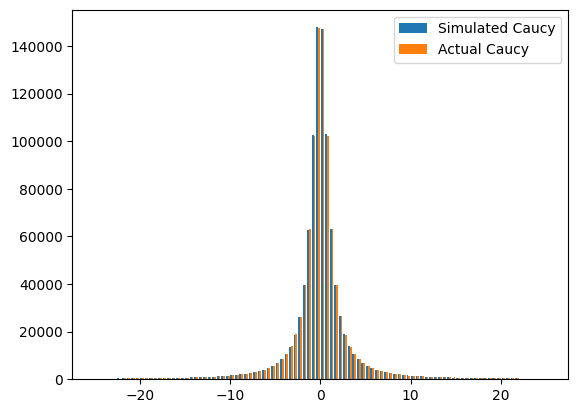
\includegraphics[width=0.8\textwidth]{cauchy.png}
		\caption{Histograma de la variable aleatoria Cauchy}
	\end{figure}
\end{homeworkProblem}

% Homework problem 2
\begin{homeworkProblem}
	Demueste como generar una variable aleatoria $X \sim DoubleExp(\mu,\beta)$ a partir de una variable aleatoria $u \sim unif(0,1)$.
	\begin{enumerate}
		\item Proceso Matematico
		      \[
			      \begin{split}
				      f(x) & = \frac{1}{\beta} e^{-\frac{x-\mu}{\beta} + e^{-\frac{x-\mu}{\beta}}} \\
				      F_X(x) & = \int_{-\infty}^{x} f(x) dx \\
				      F_X(x) & = \int_{-\infty}^{x} \frac{1}{\beta} e^{-\frac{x-\mu}{\beta} + e^{-\frac{x-\mu}{\beta}}} \\
				      F_X(x) & = e^{-e^{-\frac{x-\mu}{\beta}}} \\
				      u & = e^{-e^{-\frac{x-\mu}{\beta}}} \\
				      \log(-\log(u)) & = -\frac{x-\mu}{\beta} \\
				      \beta \log(-\log(u)) + \mu & = x \\
				      x &= \beta \log(-\log(u)) + \mu
			      \end{split}
		      \]
		\item algorithms
		      \begin{enumerate}
			      \item Generar $u \sim U(0,1)$
			      \item Definir $x = \beta \log(-\log(u)) + \mu$
		      \end{enumerate}
		\item Graphicas
		      \begin{lstlisting}[language=Python,caption=Generacion de variable aleatoria DoubleExp]
import numpy as np
import matplotlib.pyplot as plt

rng = np.random.default_rng(seed=787)
x = rng.uniform(0,1,1000000)
mu, beta = 0, 0.1 

data = beta*(-np.log(-np.log(x))+mu)
data = data[(data>-1) & (data<1)]
            \end{lstlisting}
	\end{enumerate}
	\begin{lstlisting}[language=Python, caption=Grafica de la variable aleatoria DoubleExp]
s = rng.gumbel(mu, beta, 1000000)
s = s[(s>-1) & (s<1)]


plt.hist([data, s], bins=100, label=['Simulated Gumbel ', 'Actual Gumbel'])
plt.legend(loc='upper right')
plt.show()
\end{lstlisting}

	\begin{figure}[H]
		\centering
		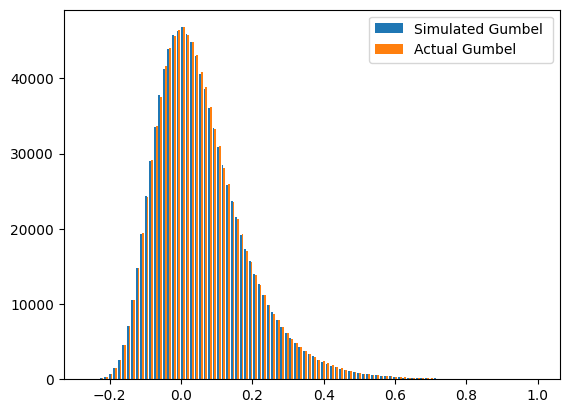
\includegraphics[width=0.8\textwidth]{doubleexp.png}
		\caption{Histograma de la variable aleatoria DoubleExp}
	\end{figure}

\end{homeworkProblem}

\end{document}


